\documentclass[10pt,journal,cspaper,compsoc]{IEEEtran}
%
% If IEEEtran.cls has not been installed into the LaTeX system files,
% manually specify the path to it like:
% \documentclass[12pt,journal,compsoc]{../sty/IEEEtran}

\usepackage{fixltx2e}
% \usepackage{stfloats}
\usepackage{amsmath}
\usepackage{graphicx}
\usepackage{amsfonts}
\usepackage{amsthm}
\usepackage{cite}
\usepackage{algorithm}
\usepackage{algorithmic}
\usepackage{url}
\input{/Users/jovo/Research/latex/latex_commands.tex}
\hyphenation{op-tical net-works semi-conduc-tor}


\begin{document}

\title{Bayes Optimal Unlabeled Graph Classification: Applications in Statistical Connectomics}

\author{Joshua T.~Vogelstein %, Mark Dredze, R.~Jacob~Vogelstein, 
 and 
Carey~E.~Priebe% <-this % stops a space
\IEEEcompsocitemizethanks{\IEEEcompsocthanksitem J.T. Vogelstein and C.E. Priebe are with the Department
of Applied Mathematics and Statistics, Johns Hopkins University, Baltimore, MD 21218.\protect\\
% note need leading \protect in front of \\ to get a newline within \thanks as
% \\ is fragile and will error, could use \hfil\break instead.
E-mail: joshuav@jhu.edu
\IEEEcompsocthanksitem R.J. Vogelstein is with the Johns Hopkins University Applied Physics Laboratory, Laurel, MD, 20723.}% <-this % stops a space
\thanks{}}
 
% The paper headers
\markboth{IN PREP}%
{Graph Classification}

\IEEEcompsoctitleabstractindextext{%
\begin{abstract}
	Graph classification algorithms often do not incorporate vertex label information in their classifiers.  In this work, we investigate the extent to which discarding vertex labels can hinder classification performance, and for which random graph models it would be expected to matter.  Via theory we demonstrate a collection of results.  Specifically, if one ``shuffles'' the graphs prior to classification, the vertex label information is irretrievably lost, which can degrade misclassification performance (and does whenever the vertex labels have class-conditional signal).  Thus, while one cannot hope to recover the labels, trying to recover the labels actually results in a consistent estimate of the optimal graph invariant.  This approach therefore solves the question of ``which invariant to use'' for any graph classification problem, at least asymptotically.  Via simulation we demonstrate that a finite (and small) number of training samples can be sufficient to achieve this bound.  Finally, we apply this approach to a ``connectome'' classification problem (a connectome is the complete set of connections within a brain).  Unshuffling the graphs indeed improves performance, although not over the best performance achievable composing a number of graph invariant and machine learning tools.  Thus, given any unlabeled graph classification problem, the relative performance of an unshuffling approach might be difficult to predict with small sample sizes.
\end{abstract}

% Note that keywords are not normally used for peer review papers.
\begin{keywords}
statistical inference, graph theory, network theory, structural pattern recognition, connectome.
\end{keywords}}


% make the title area
\maketitle
\IEEEdisplaynotcompsoctitleabstractindextext
\IEEEpeerreviewmaketitle



\section{Introduction}

\IEEEPARstart{T}{his}  work addresses graph classification with and without vertex labels.  Consider the following idealized scenario. Let $\GG: \Omega \mapsto \mc{G}_n$ be a graph-valued random variable taking values $G\in \mc{G}_n$. 
%Let each graph be a tuple, $G=(\mc{V},\mc{E}_{\mc{V}})$, where $\mc{V}$ is a set of edges $|\mc{V}|=n_v$ vertices, and $\mc{E}_{\mc{V}}=\{(u,v) : (u,v) \in \mc{E}_{\mc{V}}; u,v \in \mc{V}\}$ is a set of $|\mc{E}_{\mc{V}}|=n_e$ edges. 
Let $Y$ be a categorical random variable, $Y: \Omega \mapsto \mc{Y} \subseteq \mathbb{Z}$, such that each graph has an associated class.  A graph classifier $h: \mc{G}_n \mapsto \mc{Y}$ is any function that maps from graph space to class space.  The \emph{risk} of a classifier is the expected misclassification rate, $L_h=\EE[h[G]\neq Y]$.  The optimal classifier is the classifier that minimizes risk:
\begin{align}
	h^* = \argmin_{h \in \mc{H}} \EE[h(\GG) \neq Y].
\end{align}
where $\mc{H}$ is the set of possible classifiers.  Let $L^*=L_{h^*}$ indicate minimal (optimal) risk.  

Graph classification differs from classification of vector-valued random variables in several key aspects.  First, the structure of a graph may encode information.  Second, the vertex labels may or may not be observed.  In unobserved scenarios, NP-hard problems rear their ugly heads \cite{Conte04}.

\section{Graph Shuffling} % (fold)
\label{sec:graph_shuffling}

% section graph_shuffling (end)

Let $G$ and $G'$ be isomorphic to another if and only if $\exists \, \sigma[G]=G'$, where  $\sigma: \mc{G}_n \mapsto \mc{G}_n$ is a vertex permutation function.   An \emph{unlabeled graph} is actually a set: $\mt{G}=\{\sigma[G]: \forall \sigma \in \Sigma_n\}$, where $\Sigma_n$ is the set of permutation functions on $n$ vertices. Let $\mt{\mc{G}}_n$ be unlabeled graph space. A \emph{shuffle channel}, $\mc{C}: \mc{G}_n \mapsto \mt{\mc{G}}_n$ is a channel that takes as input a graph, uniformly at random selects a permutation function $\sigma \in \Sigma_n$, and outputs an unlabeled graph.  Let $\mt{h}: \mt{\mc{G}}_n \mapsto \mc{Y}$ be an unlabeled graph classifier, and $\mt{L}^*$ be the unlabeled optimal risk for the unlabeled optimal classifier, $\mt{h}^*$. %In this manuscript, we prove several results relating $L^*$ and $\mt{L}^*$.

\section{Model Based Graph Classifiers} % (fold)
\label{sec:model_based_graph_classifiers}

% section model_based_graph_classifiers (end)

Let $\PP=\PP_{\GG,Y}$ indicate a joint distribution of graphs and classes. This joint distribution may be decomposed into the product of a likelihood and prior term: $\PP_{\GG,Y} = \PP_{\GG|Y}\pi_Y$.  Let $\pi_y$ denote class prior probabilities, $P[Y=y]\overset{\triangle}{=}P[\{\omega: Y(\omega)=y\}]$, and let $\PP_{\GG | Y = y}=\PP_y$ denote the class-conditional distribution.  Assuming the data were sampled from a distribution, $\PP_{\GG,Y}$, a Bayes classifier which chooses the maximum a posteriori class is optimal \cite{DGL}:
\begin{align} \label{eq:bayes}
	 h^*[G] = \argmax_{y \in \mc{Y}} \PP_y \pi_{y}.
\end{align}

Let $\mt{\PP}=\PP_{\mt{\GG},Y}$ indicate the joint distribution of unlabeled (or shuffled) graphs and classes.  In other words, $\mt{\PP}$ is the same as $\PP$ except that the graphs have been passed through a shuffle channel, so $\PP$ is a distribution over graphs, and $\mt{\PP}$ is a distribution over sets of isomorphic graphs.  A Bayes optimal unlabeled graph classifier is:
\begin{align} \label{eq:unbayes}
	 \mt{h}^*[\mt{G}] = \argmax_{y \in \mc{Y}} \PP_{\mt{\GG} | Y=y} \PP_{Y=y}.
\end{align}
Let $L^*$ and $\mt{L}^*$ be the Bayes risk and unlabeled Bayes risk, under $\PP$ and $\mt{\PP}$, respectively.

It may be illustrative to consider the class-conditional distributions of graphs as a categorical distribution: $\PP_{y}[G]=\text{Cat}(G; \bth_y)$, where $\bth_y=(\theta_1,\ldots, \theta_{d})$, and $\theta_i\geq 0, \, \sum_{i \in [d]} \theta_i=1$, $d=|\mc{G}_n|$ and $[d]=\{1,2,\ldots,d\}$. After passing $\GG$ through a shuffle channel, all graphs that were isomorphic to one another must have the same probability (because the shuffle channel samples a permutation uniformly at random from $\Sigma_n$).  The distribution resulting from passing $\GG$ through a shuffle channel can therefore also be thought of as a categorical distribution, but over sets of isomorphic graphs,  $\mt{\PP}_y[\mt{G}]=\PP_{\mt{\GG} | Y=y}[\mt{G}]=\text{Cat}(\mt{G}; \mb{\eta}_y)$, where $\mb{\eta}_y=(\mb{\eta}_1,\ldots, \mb{\eta}_{\mt{d}})$, with similar constraints on $\mb{\eta}_y$ as $\bth_y$.  Note that in general $\mt{d}\ll d$.  

Thus, the effect of passing $\GG$ through a shuffle channel is to change $\bth$ such that graphs isomorphic to one another have identical probabilities, that is $\{\theta_i=\eta_j \, \forall i : G_i \in \mt{G}_j\}$.  Prior to shuffling, there is no such constraint.


% \section{Results} % (fold)
% \label{sec:results}

\section{Shuffling Can Degrade Optimal Performance} % (fold)
\label{sub:pre_and_post_shuffled_bayes_optimal_performance}

% subsection pre_and_post_shuffled_bayes_optimal_performance (end)
The result of passing the graph through a shuffle channel can only degrade, but not improve, Bayes risk, as proven below.


\begin{thm}
Assuming $(\GG,Y) \sim \PP_{\GG,Y}$, 	$L^* \leq \mt{L}^*$
\end{thm}

\begin{proof}
Let $\PP[\GG=G | Y=y]=\PP_y[\GG=G]=\PP_y[G]$, where $\PP_y[G]\geq 0$ and $\sum_{G \in \mc{G}_n} \PP_y[G]=1$. Therefore:
\begin{align}
	L^*&=\EE[h^*(\GG)\neq Y]= \int_{\mc{G}_n}\II\{h^*(\GG) \neq Y\} d\PP \nonumber
	\\&=\sum_{G \in \mc{G}_n} \min_y \PP_y[G]
\end{align}
where  $\II\{\cdot\}$ is the indicator function taking value unity whenever its argument is true and zero otherwise.  When the graphs are shuffled, we have:
\begin{align}
	\mt{L}^*&=\sum_{G \in {\mc{G}}_n} \min_y \PP_y[\sigma[G] = G]
	% \nonumber \\&
	=\sum_{G \in {\mc{G}}_n} \min_y \PP_y[\sigma[G]  \in \mt{G}]
	\nonumber \\&=\sum_{\mt{G} \in \mt{\mc{G}}_n} \min_y \PP_y[G \in \mt{G}]
\end{align}
The result follows from the fact that $\min_y \PP_y[G \in \mt{G}] \geq \min_y \PP_y[\GG=G]$ for all $G \in \mc{G}_n$.
\end{proof}

\section{When Shuffling Necessarily Degrades Bayes Optimal Performance} % (fold)
\label{sub:labels_contain_information}

% subsection labels_contain_information (end)

The above proof demonstrates that shuffling can degrade Bayes risk, but not necessarily.  A natural follow-up question is: ``under what circumstances does shuffling degrade Bayes risk?''  Below we prove that if the labels contain any class-conditional signal, then shuffling necessarily degrades Bayes risk.  We write  $\PP_{\mt{\GG}|Y} =\PP_{\GG|Y}$ if and only if $\PP[G' \in \mt{G}| Y]=\PP[\GG=G'|Y] $ for all $ G' \in \mc{G}_n$.  In other words, $\PP_{\mt{\GG}|Y}=\PP_{\GG|Y}$ if and only if $\{\theta_i=\eta_j \, \forall i : G_i \in \mt{G}_j\}$.

 When shuffling changes the distribution of graphs, such that it was the case that $\{\theta_i \neq \eta_j \, \forall i : G_i \in \mt{G}_j\}$ prior to shuffling, then shuffling necessarily degrades misclassification performance.

\begin{thm}
Assume $\pi_y=1/|\mc{Y}| $ for all $ y \in \mc{Y}$ without loss of generality.  If $\PP_{\mt{\GG}|Y} \neq \PP_{\GG|Y}$ then $L^* < \mt{L}^*$ (note the strictly less than).
\end{thm}

\begin{proof}
If $\PP_{\mt{\GG}|Y} \neq \PP_{\GG|Y}$, then it must be the case that for at least one $G'\in \mc{G}_n$ such that $\PP_y[\GG=G'] \neq \PP_y[G' \in \mt{\GG}]$.  Thus, for all $G' \in \mt{G}'$, $\min_y \PP_y[G' \in \mt{G}] > \min_y \PP_y[\GG=G']$, which implies that:
\begin{align}
	L^*=\sum_{G \in \mc{G}_n} \min_y \PP_y[G] < &\sum_{\mt{G} \in \mt{\mc{G}}_n} \min_y \PP_y[G \in \mt{G}] = \mt{L}^*.
\end{align}
\end{proof}




\section{Bayes Optimal Graph Classification After Shuffling} % (fold)
\label{sec:bayes_optimal_graph_classification_after_shuffling}

If the graph $G$ has been passed through a shuffle channel, and one still desires to classify it, one might consider two complementary approaches.  First, one might try to ``unpermute'' the graph, to recover the vertex labels, and then use a Bayes optimal graph classifier.  Second, one might try to use a graph-invariant based classifier.  A graph invariant is any function: $\psi: \mc{G}_n \mapsto \Real^d$ such that $\psi(G)=\psi(\sigma(G))$ for all $\sigma \in \Sigma_n$ and $G \in \mc{G}_n$.  A graph invariant based classifier first projects a graph into an invariant space and then classifies.  The Bayes optimal graph invariant classifier minimizes risk over all invariants: 
\begin{align}
	h^*_{\psi}=\argmin_{h_{\psi} \in \mc{H}_{\psi}} \EE[h_{\psi}(\GG)\neq Y],
\end{align}
and $L^*_{\psi}$ is the Bayes invariant risk.  


Below we show two seemingly contradictory results.  First, trying to recover the vertex labels is futile: it cannot be done.  Second, it is optimal.

\begin{thm}
After passing a graph through a shuffle channel, $\mc{C}(G)=\mt{G}$, all graphs in $\mc{G}$ are equally likely to have given rise to $\mt{G}$.
\end{thm}

\begin{proof}
The number of different permutation functions $|\Sigma_n|$ is also the number of graphs within an isomorphism class, $|\mt{G}|$.  A shuffle channel samples a permutation function uniformly at random from $\Sigma_n$.  Thus, once $G$ is shuffled, the probability of any graph $G$ giving rise the the unlabeled graph $\mc{G}$ is $1/|\mt{G}|$.  
\end{proof}

Thus, there is no hope to recover the original graph.  Yet, once the graph has been shuffled, a Bayes optimal unlabeled graph classifier cannot be beat.

\begin{thm}
After passing a graph through a shuffle channel, $L\geq \mt{L}^*$.
\end{thm}

\begin{proof}
After passing a graph through a shuffle channel, the effect on the graph distribution is a normalizing of likelihoods. Specifically, $\PP_y[\sigma(G)]=\PP_y[G]$ for all $\sigma \in \Sigma_n$ and $G \in \mc{G}_n$.  Thus, $\mt{\PP}_y[\mt{G}] \propto \PP_y[G]$ and
\begin{align}
	\argmax_{y\in\mc{Y}} \PP[\mt{\GG}=\mt{G}|Y=y] = \argmax_{y \in \mc{Y}}\PP[\GG=G|Y=y]
\end{align}  
\end{proof}

In other words, $\mt{L}^*=L^*_{\psi}$, that is, the Bayes unlabeled graph classifier is the optimal invariant-based classifier.

\section{A consistent and efficient unshuffling-based classifier} % (fold)
\label{sec:bayes_optimal_graph_invariant_based_classifier}

The above results show that after passing a graph through a shuffle channel, although nothing can be gained trying to unpermute the vertices, classifying the unlabeled graphs is optimal.  Here, we show that we can induce a consistent and efficient classifier from training data, that is, a classifier can be estimated that is asymptotically guaranteed to be optimal.

Assume that a collection of $n$ graph/class pairs are sampled independently and identically from some true but unknown distribution, $(\GG_i,Y_i) \iid \PP_{\GG,Y}=\PP_Y \pi_Y$, and that each graph has been passed through a shuffle channel.  The \emph{training data} is therefore  $\mc{T}_n=\{(\mt{\GG}_i,Y_i)_{i\in[n]}$. 
%$[\cdot; \bth]$, where $\bth \in \bTh$ is a parameter.  Note that $\PP_{\GG,Y}(\cdot; \bth)$ is but one of a (possibly infinite) set of distributions, collectively comprising the model:  $\mc{P}_{\GG,Y}=\{\PP_{\GG,Y}(\cdot; \bth) : \bth \in \bTh\}$, where $\bTh$ is the set of feasible parameters. 
In a slight abuse of notation, an \emph{induced unlabeled graph classifier}, $h: \mt{\mc{G}}_n \times (\mt{\mc{G}}_n \times \mc{Y})^n \mapsto \mc{Y}$ aims to estimate $h^*$ from the training data. A Bayes plugin unlabeled graph-classifier estimates the likelihood and prior terms and plugs them in to Eq. \eqref{eq:unbayes}
\begin{align}
	\mh{h}_{BPI}[G]=\argmax_{y\in\mc{Y}} \mh{\PP}_{\mt{\GG}|Y=y}[G]\mh{\pi}_y
\end{align}
Given consistent estimators for $\PP_y[G]$ and $\pi_Y$, the Bayes plugin classifier is also consistent \cite{DGL}.  Formally, if $\mh{\PP}_y[G] \conv \PP_y[G]$ and $\mh{\pi}_Y\conv \pi_Y$ as $n \conv \infty$, then $\mh{h}_{BPI}\conv h^*$ as $n\conv \infty$.

As described above, the class-conditional distributions of unlabeled graphs can be characterized as  categorical distributions, $\PP_{\mt{\GG}|Y=y}=\text{Cat}(\mb{\eta}_y)$.  Because a categorical distribution is in the exponential family, the maximum likelihood estimate for its parameters are exist, are unique, consistent, and efficient.  Moreover, the class prior can also be represented as a categorical random-variable, and therefore has the same properties.  Taken together, these results demonstrate that the Bayes plugin unlabeled graph classifier is consistent and efficient.

\section{A Practical Approach to Unlabeled Graph Classification} % (fold)
\label{sec:a_practical_approach_to_unlabeled_graph_classification}

While the likelihood parameters are available, estimating them requires first solving a computationally hard problem.  Specifically, to estimate each $\eta_j$ one must first determine whether each additional graph is isomorphic to a previously observed graph.  Graph isomorphism is not known to be in P or NP,  which means there is no known algorithm for solving it in polynomial time (in the worst case).  Thus, the above consistent result depends on solving an infinite number of NP problems!  While this sounds bad, in practice, many graph isomorphism algorithms are available, including approximate ones \cite{Conte04}.  

To demonstrate the practically of an isomorphism-based unlabeled graph classifier, consider an independent-edge random graph model, where the class-conditional probability of an edge is given by $\PP[A_{uv}|Y=y]=\PP_{uv|y}$, yielding a likelihood factorization: $\PP_y=\prod_{uv}\PP_{uv|y}$. Thus, the class-conditional likelihood is given by a matrix, $\PP_y \in (0,1)^{n \times n}$. We sample $s+1$ labeled graph/class pairs identically and independently from the above distribution ($s$ training samples, and 1 test sample). Then, we pass each training graph through a shuffle channel, yielding $\{\mt{G}_i\}_{i \in [s]}$.

Our classifier  proceeds as follows.  Try to match each training graph to the test graph using some graph matching strategy, yielding a estimated labeled graph for each training graph, $\mh{G}_i=f(G,\mt{G}_i)$.  We  use a quadratic assignment problem (QAP) approximate algorithm as described in \cite{VP11QAP}.  This is an approximate graph matching algorithm; while solving graph matching is NP-hard \cite{Conte04}, this approach scales cubically in $n$.  Nonetheless, we find it to be very effective.

Given the estimated labeled graphs, use $\{\mh{G}_i\}_{i \in [s]}$ to estimate the class conditional likelihood parameters using a robust L-estimator as described in \cite{VP11sigsub}, and obtain maximum likelihood estimates of the prior probabilities.  Now, we can use a Bayes plugin classifier:
\begin{align}
	\mh{h}_{BPI}[G]=\argmax_{y\in\mc{Y}} \prod_{uv} \mh{\PP}_{uv|y}\mh{\pi}_y.
\end{align}
Figure \ref{fig:1} shows the performance of this Bayes plugin classifier as a function of the number of training samples.  As we had hoped, performance monotonically increases towards optimal performance (gray dot), even though the graph matching algorithm we used was approximate, and only $\mc{O}(n^3)$ instead of exponential.

\begin{figure}[htbp]
	\centering
		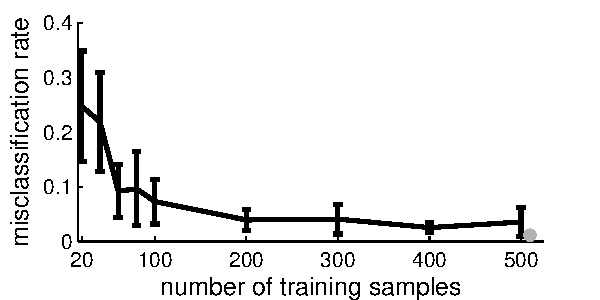
\includegraphics[width=1.0\linewidth]{../figs/hetero_easy_n10_MC5000_QAP_vs_n.pdf}
	\caption{Inexact graph matching can be used to approximate a consistent unlabeled graph classifier.  Data in this simulation was sampled from the independent edge model described above, with $\PP_{uv|0}$=Uniform$(0,0.7)$, and $\PP_{uv|1}=\PP_{uv|0}+0.3$ for all $(u,v)$; $\pi_0=\pi_1=0.5$.  For each number of training samples, we tested using 5000 test samples, and repeated 10 times.  The gray dot indicates Bayes optimal performance.}
	\label{fig:1}
\end{figure}

% section a_practical_approach_to_unlabeled_graph_classification (end)


% section bayes_optimal_graph_invariant_based_classifier (end)


\section{Unlabeled Connectome Classification} % (fold)
\label{sub:connectome_classification}

Inspired by the simulated performance of our unlabeled graph classifier, we decided to try it on a real-world application.  A ``connectome'' is a graph in which vertices correspond to biological neural units, and edges correspond to connections between the units.  Diffusion Magnetic Resonance (MR) Imaging and related technologies are making the acquisition of MR connectomes routine \cite{Hagmann2010}.  49 subjects from the Baltimore Longitudinal Study on Aging comprise this data, with acquisition and connectome inference details as reported in \cite{Gray11}.  Each connectome yields a $70 \times 70$ element binary adjacency matrix.  Associated with each graph is class label based on the gender of the individual (24 males, 25 females).  Because the vertices are labeled, we can compare the results of having the labels and not having the labels.  A $k_n$ nearest neighbor ($k$nn) classifier is universally consistent, that is, guaranteed to achieve optimal performance in the limit \cite{Stone77}, and therefore seems more appropriate than an independent edge model.  Performance is evaluated with leave-one-out misclassification rate and reported in Table \ref{tab:connectome}. When using the vertex labels, a standard $k$nn achieves $20\%$ misclassification rate.  Chance performance (only using the estimated prior) on this data is $49\%$.  These two numbers provide bounds on performance.  When all graphs are passed through a shuffle channel, we first try to unshuffle the graphs using the above mentioned QAP algorithm.  Given the unshuffled graphs, performance changes to $45\%$, not particularly impressive.  The performance of the independent edge model based Bayes plugin classifier for unlabeled graphs is similarly unimpressive.  We therefore develop a hybrid approach in which the independent edge model is assumed, and parameters are estimated using the vertex labels.  Given these estimates, we can use the QAP algorithm to match each test graph to the two likelihood matrices, and then use the Bayes plugin classifier.  This approach yields a $31\%$ misclassification rate. In contrast, a ``standard'' graph invariant based approach, which computes the graph invariants from \cite{PCP11}, and plugs them into various machine learning algorithms (including the winner \cite{Dredze08}), yields misclassification rates as low as $25\%$. 


% 
% \begin{itemize}
% 	\item \textbf{Graph Classifier} A Bayes plugin graph classifier as described in \cite{VP11a}, that is, using the labels.
% 	\item \textbf{1-QAP} Estimate the parameters using training data \emph{with} vertex labels.  Then, shuffle the test graph, \qap it to each $\mh{\PP}_y$ matrix.  The  estimated the class is $\mh{y}=\argmax_{y \in \mc{Y}}QAP(G,\mh{\PP}_y)$.   
% 	\item \textbf{48-QAP} Permuting the vertex labels, then implement \texttt{$1$NN$\circ$\qapa}.
% 	% \item \textbf{AVG-QAP}  Permuting the vertex labels, \qapa each of the 48 training graphs to the test graph.  Then, given those permuted adjacency matrices, compute the average, and then implement a standard $1$NN classifier.
% 	\item \textbf{1NN-GI} Use the graph invariant approach as described above. We provide the normalized graph invariants as inputs into a number of standard classifiers, including $k$NN, linear classifiers, support vector machines, random forests, and CW. On this data, the CW classifier performed best; we therefore only report its results.
% \end{itemize}
% 

\begin{table}[h!]
\caption{MR Connectome Leave-One-Out Misclassification Rates}
\begin{center}
\begin{tabular}{|r|r|r|r|r|}
\hline
\texttt{N/A-QAP} & \texttt{1-QAP} & \texttt{48-QAP} & \texttt{1NN-GI}\\
\hline
$20\%$ & $31\%$ & $45\%$  & $25\%$ \\
    \hline
\end{tabular}
\end{center}
\label{tab:connectome}
\end{table}%


\section{Discussion}

In this work, we have address both the theoretical and practical limitations of classifying graphs with and without including labels.  Specifically, we show that shuffling the vertex labels results in an irretrievable situation, with a possible degradation of classification performance, and a necessary degradation if the vertex labels contained class-conditional signal.  Moreover, although one cannot hope to recover the vertex labels, estimating them yields an asymptotically optimal classifier.  This suggest that efforts to estimate the vertex labels may yield useful classification results, outperforming ``standard'' graph-invariant based classifiers.  Via simulation we show that an approximate graph matching algorithm converges to the optimal performance with only about 500 training samples for a particular independent edge random graph model.   Finally, we demonstrate with connectome data that estimating the vertex labels can be useful, but that there remains room to grow to exceed misclassification performance of a carefully chosen graph invariant $\circ$ machine learning based approach on this data.   These connectome data, much like other collections of graphs, can also be equipped with both vertex and edge attributes.  As such, we hope to extend the results herein to consider the more general cases.








% use section* for acknowledgement
\ifCLASSOPTIONcompsoc
  % The Computer Society usually uses the plural form
  \section*{Acknowledgments}
\else
  % regular IEEE prefers the singular form
  \section*{Acknowledgment}
\fi


% Can use something like this to put references on a page
% by themselves when using endfloat and the captionsoff option.
\ifCLASSOPTIONcaptionsoff
  \newpage
\fi


\bibliography{/Users/jovo/Research/latex/library}
\bibliographystyle{IEEEtran}

\begin{IEEEbiography}{Joshua T. Vogelstein}
Joshua T. Vogelstein is a spritely young man, engorphed in a novel post-buddhist metaphor.

\end{IEEEbiography}


% insert where needed to balance the two columns on the last page with
% biographies
%\newpage


\begin{IEEEbiography}{Carey E. Priebe}
Buddha in training.
\end{IEEEbiography}

% Can be used to pull up biographies so that the bottom of the last one
% is flush with the other column.
% \enlargethispage{-5in}

\end{document}



